\documentclass[12pt,a4paper]{article}

% Encoding, fonts, and geometry
\usepackage[utf8]{inputenc}
\usepackage[T1]{fontenc}
\usepackage{lmodern}
\usepackage{geometry}
\geometry{margin=2.5cm}

% Math and related packages
\usepackage{amsmath,amssymb,amsthm,mathtools}
\usepackage{bm}
\usepackage{braket}
\usepackage{siunitx}

% Graphics and plots
\usepackage{graphicx}
\usepackage{tikz}
\usepackage{tikz-3dplot}
\usepackage{pgfplots}
\pgfplotsset{compat=1.18}
\usetikzlibrary{arrows.meta,positioning,shapes,calc,angles,quotes,patterns,3d,decorations.fractals,shadows}

% Tables, code, floats, lists
\usepackage{booktabs}
\usepackage{listings}
\usepackage{xcolor}
\usepackage{algorithm}
\usepackage{algorithmic}
\usepackage{multicol}
\usepackage{enumitem}

% Boxes
\usepackage{tcolorbox}

% Hyperlinks and clever references
\usepackage{hyperref}
\usepackage{cleveref}

% Theorem environments
\newtheorem{theorem}{Theorem}
\newtheorem{lemma}{Lemma}
\newtheorem{corollary}{Corollary}
\newtheorem{definition}{Definition}
\newtheorem{axiom}{Axiom}
\newtheorem{proposition}{Proposition}
\newtheorem{remark}{Remark}
\newtheorem{assumption}{Assumption}

% Operators
\DeclareMathOperator{\Tr}{Tr}
\DeclareMathOperator{\Diff}{Diff}
\DeclareMathOperator{\Aut}{Aut}
\DeclareMathOperator{\Vol}{Vol}
\DeclareMathOperator{\Ric}{Ric}
\DeclareMathOperator{\Riem}{Riem}
\DeclareMathOperator{\Cov}{Cov}
\DeclareMathOperator{\supp}{supp}
\DeclareMathOperator{\diag}{diag}
\DeclareMathOperator{\sign}{sign}
\DeclareMathOperator{\dimension}{dim}
\DeclareMathOperator{\Div}{Div}
\DeclareMathOperator{\Grad}{Grad}
\DeclareMathOperator{\Hess}{Hess}
\DeclareMathOperator{\Ricci}{Ricci}
\DeclareMathOperator{\Scalar}{Scalar}

% Robust math shorthands
\DeclareRobustCommand{\alD}{\texorpdfstring{\ensuremath{\alpha_{\mathrm{D}}}}{alpha_D}}
\DeclareRobustCommand{\beI}{\texorpdfstring{\ensuremath{\beta_{\mathrm{I}}}}{beta_I}}
\DeclareRobustCommand{\gaR}{\texorpdfstring{\ensuremath{\gamma_{\mathrm{R}}}}{gamma_R}}
\DeclareRobustCommand{\UCS}{\texorpdfstring{\ensuremath{\mathcal{M}_{\mathrm{UCS}}}}{M_UCS}}

% YUCT-specific commands
\newcommand{\eff}{\mathrm{eff}}
\newcommand{\coord}{\mathrm{coord}}
\newcommand{\Yak}{\mathrm{Yak}}
\newcommand{\Dict}{\mathcal{D}}
\newcommand{\Mdict}{\mathcal{M}_{\Dict}}
\newcommand{\Ke}{K_{\eff}}
\newcommand{\Kemax}{K_{\eff,\max}}
\newcommand{\Keobs}{K_{\eff,\mathrm{obs}}}
\newcommand{\Keexp}{K_{\eff,\mathrm{exp}}}
\newcommand{\Kec}{K_{\eff,c}}
\newcommand{\Kcrit}{K_{\mathrm{crit}}}

% PDF metadata
\hypersetup{
	pdftitle={Philosophy of Consciousness within Yakushev's Unified Coordination Theory (YUCT): From the "Hard Problem" to Dynamic Dictionaries},
	pdfauthor={Alexey V. Yakushev},
	pdfsubject={Consciousness, Philosophy of Mind, YUCT, Coordination Theory, Dictionaries, Hard Problem},
	pdfkeywords={YUCT, Consciousness, Philosophy of Mind, Coordination, Dictionaries, Hard Problem, Fractal, Meta-Dictionary}
}

\begin{document}
	
	% Title page
	\begin{titlepage}
		\begin{center}
			\vspace*{0cm}
			
			\Huge\textbf{Appendix I. Philosophy of Consciousness within Yakushev's Unified Coordination Theory (YUCT):\\ From the "Hard Problem" to Dynamic Dictionaries}
			
			\vspace{1cm}
			
			\small\textit{A Philosophical Foundation for Solving the "Hard Problem" through Coordination and Dictionaries}
			
			\vspace{0.5cm}
			
			\small\textbf{Alexey V. Yakushev}
			
\vspace{1cm}
\Large
Alexey V. Yakushev\\

\url{https://yuct.org/}\\
\url{https://ypsdc.com/}

\vspace{2cm}
\large YUCT \\ 
\url{https://doi.org/10.5281/zenodo.18444599}\\
\vspace{1cm}

\vspace{0cm}
\large
January 2026

\vspace{6cm}
\textcopyright~2026 Yakushev Research. All rights reserved.

\newpage
			
			\begin{abstract}
				\noindent
				This article provides a philosophical foundation for solving the "hard problem of consciousness" within the framework of the Unified Coordination Theory (YUCT). Consciousness is understood not as an epiphenomenon or illusion, but as a \textbf{dynamic coordination process} implemented through a hierarchy of \textbf{internal dictionaries}. It is shown that the classical "brain–consciousness" dualism is overcome through a three-level model: \textbf{genetic}, \textbf{neural}, and \textbf{cultural dictionaries}. Subjective experience is interpreted as the result of \textbf{live coordination} between neural ensembles using shared semantic spaces. The meta-dictionary (the ability to reflect on one's own states) explains the phenomenon of selfhood. Philosophical implications of the theory include: (1) naturalization of consciousness without reductionism; (2) a new understanding of the evolution of mind as growth in the complexity of coordination dictionaries; (3) the possibility of non-anthropomorphic forms of consciousness; (4) connection with problems of dark matter and quantum correlation on cosmological scales. YUCT offers not only a solution to the "hard problem" but also a unified philosophical platform for dialogue between neuroscience, physics, and the humanities.
			\end{abstract}
			
			\vspace{0cm}
			
			\noindent
			\small\textbf{Keywords:} YUCT, Consciousness, Philosophy of Mind, Coordination, Dictionaries, Hard Problem, Fractal, Meta-Dictionary
			
			\vspace{0.5cm}
			
			\noindent
			\textcopyright 2026 Yakushev Research. All rights reserved.
		\end{center}
	\end{titlepage}
	
	\tableofcontents
	
	\newpage
	
	\section{Introduction: The "Hard Problem" and Critique of Classical Approaches}
	
	The "hard problem of consciousness," formulated by David Chalmers, remains a central challenge for the philosophy of mind and cognitive science. The question of \textbf{how physical processes in the brain give rise to subjective experience} (qualia) traditionally places materialism and dualism on opposite sides of the barricade.
	
	Classical approaches:
	\begin{enumerate}
		\item \textbf{Dualism} (Descartes): consciousness is a substance separate from matter.
		\item \textbf{Materialism/Reductionism}: consciousness is an epiphenomenon or illusion.
		\item \textbf{Functionalism}: consciousness is a computational process.
		\item \textbf{Panpsychism}: consciousness is a fundamental property of matter.
	\end{enumerate}
	
	YUCT proposes a \textbf{coordination approach}, avoiding both dualism and crude reductionism. Consciousness is not a "thing," but a \textbf{mode of functioning of a complex system}, achieved at high coordination efficiency ($K_{\text{eff}} \gg 1$).
	
	\section{YUCT: Consciousness as Live Coordination}
	
	\subsection{From Information Processing to Coordination}
	
	Classical cognitive sciences view the brain as an information-processing device. YUCT shifts the emphasis: \textbf{consciousness is not information processing, but live coordination between internal agents} (neural ensembles).
	
	Formally:
	\[
	\Psi(t) = D(t) + I(t) \times R(t)
	\]
	where:
	\begin{itemize}
		\item $D(t)$ – ontological dictionary (rules, categories, action patterns);
		\item $I(t)$ – informational state (entropy, complexity);
		\item $R(t)$ – resonance factor (coordination amplification coefficient).
	\end{itemize}
	
	Subjective experience arises when $R(t)$ reaches a threshold at which internal states synchronize into a unified semantic field.
	
	\subsection{Internal Dictionaries and Qualia}
	
	"Redness of red" or "pain" are not primitive atoms of experience but \textbf{complex coordination patterns} encoded in the internal sensory dictionary.
	
	\begin{tcolorbox}[title=Example: Synesthesia and Phantom Pains]
		Synesthesia ("colored hearing") and phantom pains are not anomalies but manifestations of \textbf{cross-activation of dictionaries}. Indexing errors or coordination failures between sensory dictionaries lead to modality mixing.
	\end{tcolorbox}
	
	Thus, qualia are not "raw sensations" but \textbf{high-level coordination states} arising from the activation of complex dictionary patterns.
	
	\subsection{Self-Consciousness as Meta-Dictionary}
	
	The "self" is not a homunculus or an illusion but a \textbf{meta-level of coordination}. A system capable of forming a \textbf{meta-dictionary} to describe and coordinate its own states acquires self-referentiality.
	
	Mathematically: when $K_{\text{eff}} \to \infty$ in a closed system, a self-referential loop emerges, subjectively experienced as "selfhood." This is not a "soul" but an \textbf{emergent property of highly efficient coordination}.
	
	\section{Three-Level Dictionary Model: From Genes to Memes}
	
	\begin{figure}[h!]
		\centering
		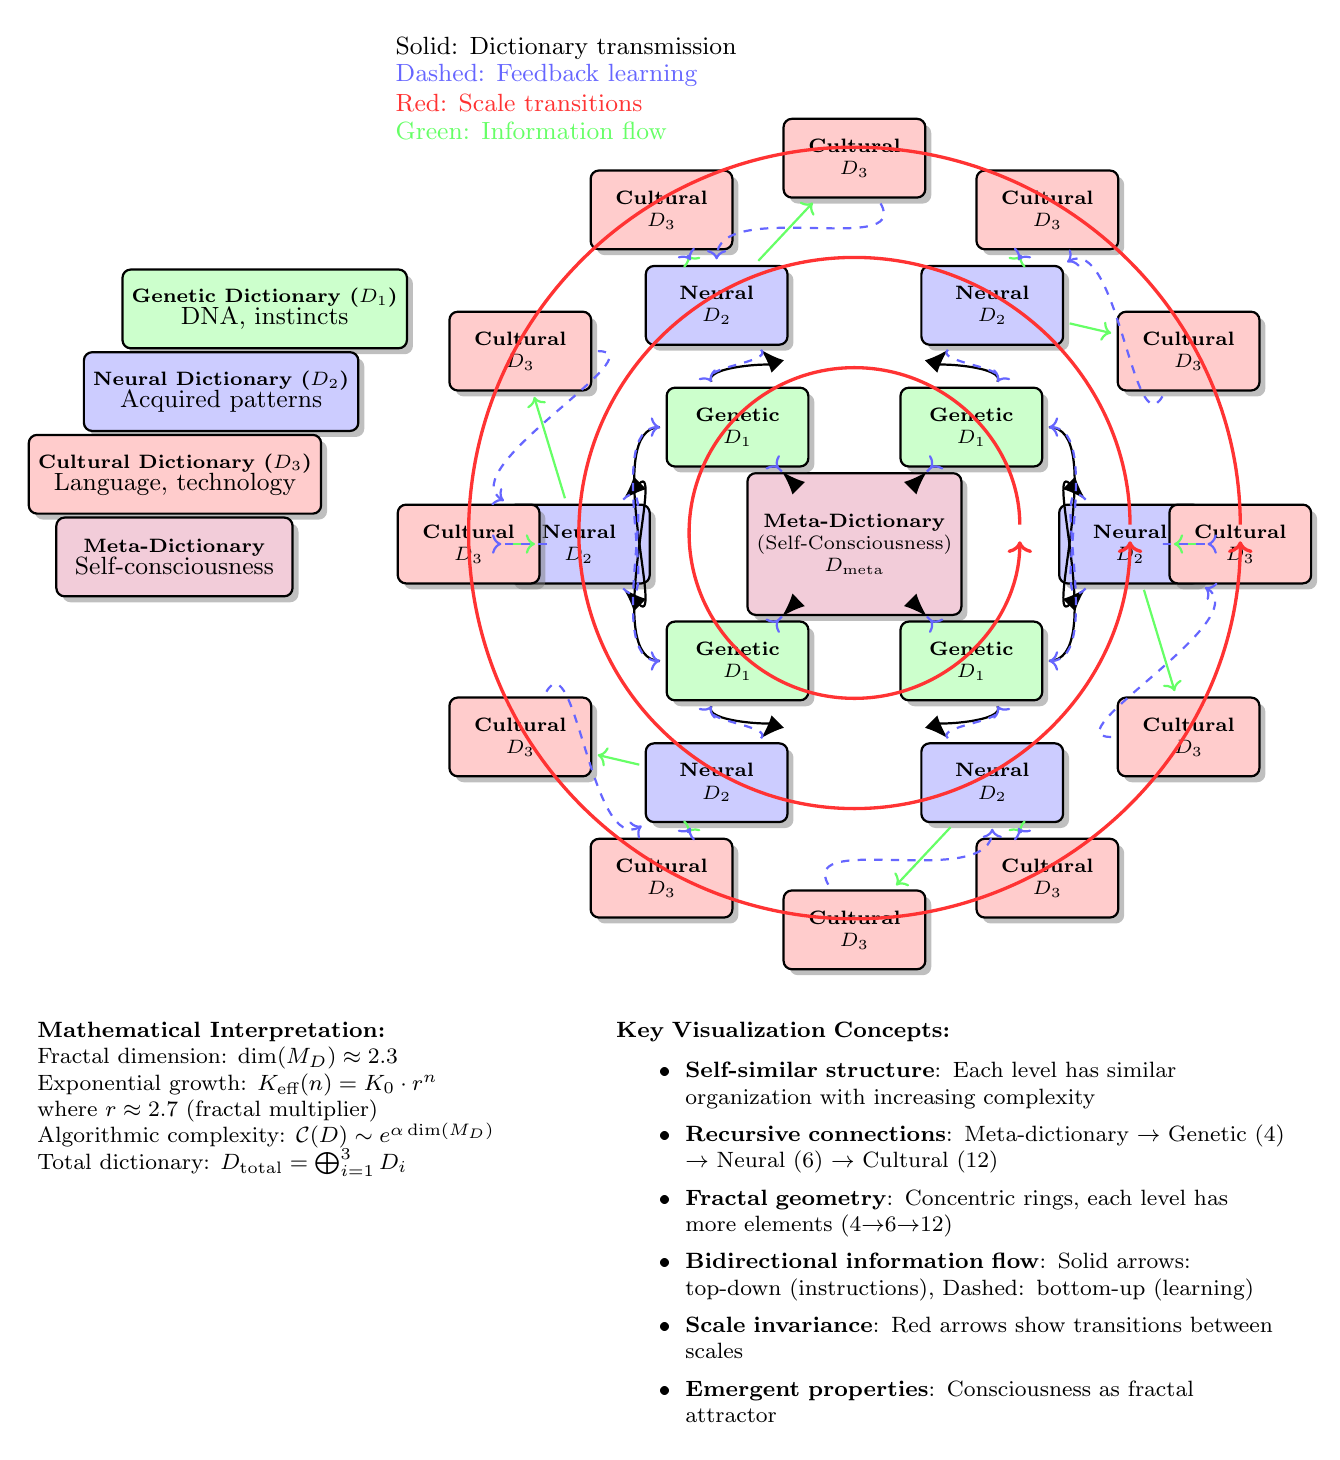
\begin{tikzpicture}[
			scale=0.7,
			dictbox/.style={
				rectangle, rounded corners=3pt, draw=black, thick,
				fill=white, drop shadow, align=center, 
				minimum width=1.8cm, minimum height=1cm,
				font=\scriptsize
			},
			level1/.style={fill=green!20},
			level2/.style={fill=blue!20},
			level3/.style={fill=red!20},
			level4/.style={fill=purple!20},
			fractalarrow/.style={-{Latex[length=3mm]}, thick, shorten >=2pt, shorten <=2pt},
			feedback/.style={->, dashed, thick, blue!60, shorten >=2pt, shorten <=2pt},
			scalearrow/.style={->, very thick, red!80, shorten >=3pt, shorten <=3pt},
			infoflow/.style={->, thick, green!60, shorten >=2pt, shorten <=2pt}
			]
			
			% Central meta-dictionary
			\node[dictbox, level4, minimum width=2.5cm, minimum height=1.8cm] (meta) at (0,0) 
			{\textbf{Meta-Dictionary}\\ (Self-Consciousness)\\ $D_{\text{meta}}$};
			
			% Genetic dictionaries (4)
			\node[dictbox, level1] (gen45) at (45:3cm) {\textbf{Genetic}\\ $D_1$};
			\node[dictbox, level1] (gen135) at (135:3cm) {\textbf{Genetic}\\ $D_1$};
			\node[dictbox, level1] (gen225) at (225:3cm) {\textbf{Genetic}\\ $D_1$};
			\node[dictbox, level1] (gen315) at (315:3cm) {\textbf{Genetic}\\ $D_1$};
			
			% Neural dictionaries (6)
			\node[dictbox, level2] (neuro0) at (0:5cm) {\textbf{Neural}\\ $D_2$};
			\node[dictbox, level2] (neuro60) at (60:5cm) {\textbf{Neural}\\ $D_2$};
			\node[dictbox, level2] (neuro120) at (120:5cm) {\textbf{Neural}\\ $D_2$};
			\node[dictbox, level2] (neuro180) at (180:5cm) {\textbf{Neural}\\ $D_2$};
			\node[dictbox, level2] (neuro240) at (240:5cm) {\textbf{Neural}\\ $D_2$};
			\node[dictbox, level2] (neuro300) at (300:5cm) {\textbf{Neural}\\ $D_2$};
			
			% Cultural dictionaries (12)
			\node[dictbox, level3] (culture0) at (0:7cm) {\textbf{Cultural}\\ $D_3$};
			\node[dictbox, level3] (culture30) at (30:7cm) {\textbf{Cultural}\\ $D_3$};
			\node[dictbox, level3] (culture60) at (60:7cm) {\textbf{Cultural}\\ $D_3$};
			\node[dictbox, level3] (culture90) at (90:7cm) {\textbf{Cultural}\\ $D_3$};
			\node[dictbox, level3] (culture120) at (120:7cm) {\textbf{Cultural}\\ $D_3$};
			\node[dictbox, level3] (culture150) at (150:7cm) {\textbf{Cultural}\\ $D_3$};
			\node[dictbox, level3] (culture180) at (180:7cm) {\textbf{Cultural}\\ $D_3$};
			\node[dictbox, level3] (culture210) at (210:7cm) {\textbf{Cultural}\\ $D_3$};
			\node[dictbox, level3] (culture240) at (240:7cm) {\textbf{Cultural}\\ $D_3$};
			\node[dictbox, level3] (culture270) at (270:7cm) {\textbf{Cultural}\\ $D_3$};
			\node[dictbox, level3] (culture300) at (300:7cm) {\textbf{Cultural}\\ $D_3$};
			\node[dictbox, level3] (culture330) at (330:7cm) {\textbf{Cultural}\\ $D_3$};
			
			% Connections from meta to genetic
			\draw[fractalarrow] (meta) -- (gen45);
			\draw[fractalarrow] (meta) -- (gen135);
			\draw[fractalarrow] (meta) -- (gen225);
			\draw[fractalarrow] (meta) -- (gen315);
			
			\draw[feedback] (gen45) to[out=225, in=45] (meta);
			\draw[feedback] (gen135) to[out=315, in=135] (meta);
			\draw[feedback] (gen225) to[out=45, in=225] (meta);
			\draw[feedback] (gen315) to[out=135, in=315] (meta);
			
			% Connections from genetic to neural
			\draw[fractalarrow] (gen45) to[out=0, in=225] (neuro0);
			\draw[fractalarrow] (gen45) to[out=60, in=225] (neuro60);
			
			\draw[fractalarrow] (gen135) to[out=120, in=315] (neuro120);
			\draw[fractalarrow] (gen135) to[out=180, in=315] (neuro180);
			
			\draw[fractalarrow] (gen225) to[out=240, in=45] (neuro240);
			\draw[fractalarrow] (gen225) to[out=180, in=45] (neuro180);
			
			\draw[fractalarrow] (gen315) to[out=300, in=135] (neuro300);
			\draw[fractalarrow] (gen315) to[out=0, in=135] (neuro0);
			
			% Feedback from neural to genetic
			\draw[feedback] (neuro0) to[out=225, in=0] (gen45);
			\draw[feedback] (neuro60) to[out=225, in=60] (gen45);
			
			\draw[feedback] (neuro120) to[out=315, in=120] (gen135);
			\draw[feedback] (neuro180) to[out=315, in=180] (gen135);
			
			\draw[feedback] (neuro240) to[out=45, in=240] (gen225);
			\draw[feedback] (neuro180) to[out=45, in=180] (gen225);
			
			\draw[feedback] (neuro300) to[out=135, in=300] (gen315);
			\draw[feedback] (neuro0) to[out=135, in=0] (gen315);
			
			% Connections from neural to cultural
			\draw[infoflow] (neuro0) -- (culture0);
			\draw[infoflow] (neuro0) -- (culture330);
			
			\draw[infoflow] (neuro60) -- (culture60);
			\draw[infoflow] (neuro60) -- (culture30);
			
			\draw[infoflow] (neuro120) -- (culture120);
			\draw[infoflow] (neuro120) -- (culture90);
			
			\draw[infoflow] (neuro180) -- (culture180);
			\draw[infoflow] (neuro180) -- (culture150);
			
			\draw[infoflow] (neuro240) -- (culture240);
			\draw[infoflow] (neuro240) -- (culture210);
			
			\draw[infoflow] (neuro300) -- (culture300);
			\draw[infoflow] (neuro300) -- (culture270);
			
			% Feedback from cultural to neural
			\draw[feedback] (culture0) to[out=180, in=0] (neuro0);
			\draw[feedback] (culture330) to[out=180, in=330] (neuro0);
			
			\draw[feedback] (culture60) to[out=240, in=60] (neuro60);
			\draw[feedback] (culture30) to[out=240, in=30] (neuro60);
			
			\draw[feedback] (culture120) to[out=300, in=120] (neuro120);
			\draw[feedback] (culture90) to[out=300, in=90] (neuro120);
			
			\draw[feedback] (culture180) to[out=0, in=180] (neuro180);
			\draw[feedback] (culture150) to[out=0, in=150] (neuro180);
			
			\draw[feedback] (culture240) to[out=60, in=240] (neuro240);
			\draw[feedback] (culture210) to[out=60, in=210] (neuro240);
			
			\draw[feedback] (culture300) to[out=120, in=300] (neuro300);
			\draw[feedback] (culture270) to[out=120, in=270] (neuro300);
			
			% Scale arrows
			\draw[scalearrow] (3,0.2) arc (0:360:3);
			\draw[scalearrow] (5,0.2) arc (0:360:5);
			\draw[scalearrow] (7,0.2) arc (0:360:7);
			
			% Legend
			\node[dictbox, level1, anchor=north west, minimum width=3cm] at (-13.3,5) 
			{\textbf{Genetic Dictionary ($D_1$)}\\\small DNA, instincts};
			\node[dictbox, level2, anchor=north west, minimum width=3cm] at (-14,3.5) 
			{\textbf{Neural Dictionary ($D_2$)}\\\small Acquired patterns};
			\node[dictbox, level3, anchor=north west, minimum width=3cm] at (-15,2) 
			{\textbf{Cultural Dictionary ($D_3$)}\\\small Language, technology};
			\node[dictbox, level4, anchor=north west, minimum width=3cm] at (-14.5,0.5) 
			{\textbf{Meta-Dictionary}\\\small Self-consciousness};
			
			% Arrow legend
			\node[anchor=west] at (-8.5,9) {\textcolor{black}{\small Solid: Dictionary transmission}};
			\node[anchor=west] at (-8.5,8.5) {\textcolor{blue!60}{\small Dashed: Feedback learning}};
			\node[anchor=west] at (-8.5,8) {\textcolor{red!80}{\small Red: Scale transitions}};
			\node[anchor=west] at (-8.5,7.5) {\textcolor{green!60}{\small Green: Information flow}};
			
			% Mathematical interpretation
			\node[anchor=north west, align=left, font=\footnotesize] at (-15,-8.5) {
				\textbf{Mathematical Interpretation:}\\
				Fractal dimension: $\dim(M_D) \approx 2.3$\\
				Exponential growth: $K_{\text{eff}}(n) = K_0 \cdot r^n$\\
				where $r \approx 2.7$ (fractal multiplier)\\
				Algorithmic complexity: $\mathcal{C}(D) \sim e^{\alpha \dim(M_D)}$\\
				Total dictionary: $D_{\text{total}} = \bigoplus_{i=1}^3 D_i$
			};
			
			% Key ideas
			\node[anchor=north west, align=left, font=\footnotesize, text width=8.5cm] at (-4.5,-8.5) {
				\textbf{Key Visualization Concepts:}\\
				\begin{itemize}
					\item \textbf{Self-similar structure}: Each level has similar organization with increasing complexity
					\item \textbf{Recursive connections}: Meta-dictionary $\to$ Genetic (4) $\to$ Neural (6) $\to$ Cultural (12)
					\item \textbf{Fractal geometry}: Concentric rings, each level has more elements (4$\to$6$\to$12)
					\item \textbf{Bidirectional information flow}: Solid arrows: top-down (instructions), Dashed: bottom-up (learning)
					\item \textbf{Scale invariance}: Red arrows show transitions between scales
					\item \textbf{Emergent properties}: Consciousness as fractal attractor
				\end{itemize}
			};
			
		\end{tikzpicture}
		\caption{Fractal structure of YUCT dictionaries illustrating the key concepts: (1) Self-similar organization across genetic ($D_1$), neural ($D_2$), and cultural ($D_3$) levels; (2) Recursive connections forming a hierarchical network; (3) Scale invariance with fractal dimension $\dim(M_D) \approx 2.3$; (4) Bidirectional information flow (solid arrows: dictionary transmission, dashed: feedback learning); (5) Exponential growth of coordination efficiency $K_{\text{eff}}(n) = K_0 \cdot r^n$ with $r \approx 2.7$. The fractal geometry explains consciousness scalability, recursive reflection (meta-dictionary), efficient inter-level information transfer, and emergent properties of consciousness as a fractal attractor.}
		\label{fig:fractal_dict}
	\end{figure}
	
	YUCT offers a unified mechanism for the continuity of consciousness across levels of organization, as illustrated in Figure~\ref{fig:fractal_dict}:
	
	\subsection{1. Genetic Dictionary ($D_1$)}
	
	DNA is a \textbf{priori dictionary} distributed within a population. The "code" is not a metaphor but a real transcription-translation process where codons are "words" and proteins are "actions."
	
	\subsection{2. Neural/Instinctive Dictionary ($D_2$)}
	
	Pre-established neural patterns (instincts, reflexes) are \textbf{hardwired coordination programs}. A sensory trigger is the "key" to activating a dictionary entry.
	
	\subsection{3. Cultural/Memetic Dictionary ($D_3$)}
	
	Language, rituals, technology are \textbf{dynamic dictionaries} transmitted through learning. A meme (according to Dawkins) in YUCT is a \textbf{package of an "index" ($\kappa$) and a "dictionary instruction" ($\Delta D$)}.
	
	The evolution of mind is the growth of $K_{\text{eff}}$ in transmitting $D_3$, exhibiting fractal properties with self-similar coordination patterns repeating across scales:
	\[
	K_{\text{eff}} \sim 
	\begin{cases}
		10^2 & \text{oral tradition}\\
		10^4 & \text{writing}\\
		10^6 & \text{printing}\\
		10^{10} & \text{internet}
	\end{cases}
	\]
	
	The fractal structure (Figure~\ref{fig:fractal_dict}) demonstrates how each dictionary level simultaneously functions as both a whole system and a component of a larger hierarchy, enabling the scalability, recursive reflection, and emergent properties characteristic of consciousness.
	
	\section{Philosophical Implications}
	
	\subsection{Naturalization Without Reductionism}
	
	YUCT offers a \textbf{naturalistic but non-reductionist} explanation of consciousness. Subjective experience is not reduced to "neural firing," nor does it require non-physical substances. It emerges as a \textbf{property of high-level coordination}, which, although implemented in neurons, is described in terms of dictionaries and resonances.
	
	\subsection{Evolutionary Meaning of Consciousness}
	
	Consciousness is not a luxury or an accidental byproduct. Evolutionary advantage comes from the \textbf{ability to form and transmit complex, flexible, compressed dictionaries} for coordinating behavior, anticipation, and cooperation. \textbf{Mind is the transmission of improved dictionaries}.
	
	\subsection{Possibility of Non-Human Consciousness}
	
	YUCT removes anthropocentric bias. Consciousness is possible in systems with high $K_{\text{eff}}$, regardless of substrate:
	\begin{itemize}
		\item Collective mind (swarm, flock)
		\item Artificial neural networks
		\item Hypothetical planetary or stellar systems
	\end{itemize}
	
	The criterion for consciousness is not "resemblance to humans" but \textbf{coordination complexity}.
	
	\subsection{Connection with Fundamental Physics}
	
	If dictionaries ($D$) are fundamental, they must have:
	\begin{itemize}
		\item \textbf{Carrier}: geometry of dictionary manifolds $M_D$ as a physical structure (possibly quantum correlations or spacetime topology).
		\item \textbf{Dynamics}: equation for $dD/dt$, as fundamental as the Schrödinger equation.
		\item \textbf{Interaction}: coordination interaction as a new type of physical interaction.
	\end{itemize}
	
	\subsection{Dark Matter/Energy as Coordination Limits}
	
	Hypothesis: on cosmological scales, $K_{\text{eff}} \to 0$ means \textbf{loss of the ability to maintain global dictionaries}. Dark energy may not be "energy" but the \textbf{limit of the Universe's coordinative connectivity}, its inability to maintain a coherent state on scales larger than the event horizon.
	
	\section{The Dilemma: Predetermination vs. Free Creation of Dictionaries}
	
	The origin of dictionaries leads to a fundamental question: are they predetermined from the Universe's birth, or freely created locally? YUCT resolves this through a hierarchical view:
	
	\subsection{Levels of Dictionaries in the Universe}
	
	\[
	\mathcal{L}_{\text{dictionaries}} = \mathcal{L}_{\text{fundamental}} + \mathcal{L}_{\text{emergent}} + \mathcal{L}_{\text{creative}}
	\]
	
	\subsubsection{1. Fundamental Dictionaries: Legacy of the Big Bang}
	
	Initial conditions encoded potential coordination patterns:
	\[
	\Psi_{\text{initial}} = \sum_{n=1}^N \alpha_n |\chi_n^{\text{fund}}\rangle
	\]
	
	These contain \textbf{all possibilities but no specific events}—like an alphabet and grammar, not a complete book.
	
	\subsubsection{2. Emergent Dictionaries: Freedom Within Rules}
	
	New dictionaries arise through evolutionary processes:
	\[
	\frac{d\chi_{\text{new}}}{dt} = \mu \cdot \nabla_{\text{old}} S_{\text{info}} \times \text{Innovation}(t)
	\]
	
	Examples: genetic code, neural networks, languages, technologies.
	
	\subsubsection{3. Creative Dictionaries: Local Innovation}
	
	Local systems create sub-dictionaries within fundamental constraints:
	\[
	\mathcal{L}_{\text{creation}} = \lambda_{\text{create}} \cdot \exp\left[-\beta \cdot D(\chi_{\text{new}} || \chi_{\text{fund}})\right] \cdot K_{\text{eff}}^{\text{creative}}
	\]
	
	\subsection{The YUCT Resolution: Complementarity Not Contradiction}
	
	YUCT proposes that fundamental dictionaries set the \textbf{alphabet} of possible states, while emergent and creative processes write the \textbf{text} of reality. This is not rigid determinism but \textbf{determinism within a space of possibilities}.
	
	Mathematically, system evolution follows:
	\[
	\frac{d}{dt}\left( K_{\text{eff}} \frac{dc}{dt} \right) = -\frac{\partial V}{\partial c} + \text{stochastic terms}
	\]
	
	where stochastic terms (quantum fluctuations, random events) introduce genuine unpredictability.
	
	\section{The Universal Pattern: Hierarchies of Self-Replicating Dictionaries}
	
	The fundamental revelation of YUCT is the fractal self-similarity across all scales of existence:
	
	\textbf{Universal Pattern:}
	\begin{center}
		Cell $\to$ Organism $\to$ Community $\to$ Civilization $\to$ Universe\\
		$\downarrow$ \hspace{1cm} $\downarrow$ \hspace{1.2cm} $\downarrow$ \hspace{1.2cm} $\downarrow$ \hspace{1.2cm} $\downarrow$\\
		Dictionary\hspace{0.5cm} Dictionary\hspace{0.5cm} Dictionary\hspace{0.5cm} Dictionary\hspace{0.5cm} Dictionary\\
		of growth\hspace{0.2cm} of behavior\hspace{0.1cm} of interaction\hspace{0.1cm} of coordination\hspace{0.1cm} of laws
	\end{center}
	
	\subsection{Examples Across Scales}
	
	\begin{itemize}
		\item \textbf{Cells:} DNA dictionary (ATG: "start", TAA: "stop", etc.)
		\item \textbf{Neurons:} Synaptic dictionary (input pattern $\to$ output pattern)
		\item \textbf{Businesses:} Business model dictionary (customer $\to$ value $\to$ profit)
		\item \textbf{Technologies:} API dictionary (request $\to$ response)
	\end{itemize}
	
	\subsection{The Law of System Survival}
	
	For any system $S$ at time $t$:
	\[
	\frac{dS}{dt} = \alpha \cdot D \cdot F - \beta \cdot E
	\]
	where $D(t)$ = number of active dictionaries, $F(t)$ = fractal complexity, $E(t)$ = system entropy.
	
	The coordination efficiency becomes:
	\[
	K_{\text{eff}}(t) = \frac{D(t) \cdot F(t)}{E(t)}
	\]
	
	\textbf{Survival rule:} If $d(\text{dictionaries})/dt > 0$, system grows ($K_{\text{eff}} \uparrow$); if $< 0$, system degrades (entropy $\uparrow$).
	
	\section{Phase Transitions via $K_{\text{eff}}$: The Engine of Complexity Evolution}
	
	$K_{\text{eff}}$ drives phase transitions between levels of organization through critical thresholds:
	
	\subsection{General Scheme of Transitions}
	
	\begin{center}
		\scalebox{0.75}{ % Масштабируем таблицу
			\begin{tabular}{|c|c|c|c|}
				\hline
				\textbf{Level} & \textbf{Phase 1 (low $K_{\text{eff}}$)} & \textbf{Phase 2 (high $K_{\text{eff}}$)} & \textbf{Order Parameter} \\
				\hline
				Quantum $\to$ Classical & Decoherence, stochasticity & Coherence, entanglement & Degree of quantum correlation \\
				\hline
				Classical $\to$ Informational & Chaotic interactions & Synchronization, protocols & Synchronization measure \\
				\hline
				Informational $\to$ Conscious & Reflexes, instincts & Goal-setting, planning & Complexity of internal model \\
				\hline
			\end{tabular}
		}
	\end{center}
	
	\subsection{1. Level 2 $\to$ 3: Quantum to Classical Transition}
	
	Governed by decoherence/coherence dynamics:
	\[
	\frac{d\rho}{dt} = -\frac{i}{\hbar}[H,\rho] + \gamma\left(L\rho L^\dagger - \frac{1}{2}\{L^\dagger L,\rho\}\right)
	\]
	
	Critical condition: $K_{\text{eff}}^{(2\to3)} = \frac{\tau_{\text{coh}}}{\tau_{\text{dec}}} > K_{\text{crit}} \approx 1$
	
	\subsection{2. Level 3 $\to$ 4: Classical to Informational Transition}
	
	Kuramoto model with $K_{\text{eff}}$:
	\[
	\dot{\theta}_i = \omega_i + \frac{K_{\text{eff}}}{N}\sum_{j=1}^N \sin(\theta_j - \theta_i)
	\]
	
	Phase transition at: $K_{\text{eff}}^{(3\to4)} > K_c = \frac{2}{\pi g(0)}$
	
	\subsection{3. Level 4 $\to$ 5: Informational to Conscious Transition}
	
	$K_{\text{eff}}$ becomes measure of integrated information $\Phi$:
	\[
	\Phi = K_{\text{eff}} \cdot I_{\text{mutual}}
	\]
	
	Critical threshold: $\Phi > \Phi_{\text{crit}} \approx 20-30$ bits (human consciousness)
	
	\subsection{Universal Mechanism: Catastrophe Theory}
	
	All transitions described by Landau potential:
	\[
	V(\psi) = \frac{\alpha}{2}(K_c - K_{\text{eff}})\psi^2 + \frac{\beta}{4}\psi^4
	\]
	
	Transition occurs at $K_{\text{eff}} > K_c$, creating new order parameter $\psi$.
	
	\subsection{Deep Meaning: $K_{\text{eff}}$ as Evolutionary Driver}
	
	The Universe evolves through $K_{\text{eff}}$-driven phase transitions:
	\[
	\frac{dK_{\text{eff}}}{dt} = \alpha K_{\text{eff}}(1 - K_{\text{eff}}/K_{\text{max}}) - \beta \nabla^2 K_{\text{eff}} + \gamma \xi(t)
	\]
	
	Each transition creates new dictionaries and enables self-reference—the essence of consciousness evolution.
	\section{The Sensory Coordination Hypothesis: From Genetic Blueprints to Direct Experience}
	
	\subsection{The Illusion of Simplicity in Sensory Perception}
	
	A fundamental puzzle in consciousness studies is why complex neurological processes are subjectively experienced as simple, immediate sensations. According to YUCT, this apparent immediacy emerges from \textbf{high-efficiency coordination ($K_{\text{eff}}$) across hierarchical dictionaries}. What we perceive as "simple redness" or "direct pain" is actually the endpoint of a sophisticated multi-level coordination process.
	
	\subsection{Genetic Dictionaries as Blueprints for Sensory Coordination}
	
	The genetic code provides not merely sensory receptors but \textbf{coordination architectures} for processing sensory information:
	
	\begin{itemize}
		\item \textbf{$D_1$ (Genetic Dictionary) encodes:}
		\begin{itemize}
			\item Receptor types and distributions (cones for color, nociceptors for pain)
			\item Basic neural pathway architectures (thalamocortical projections)
			\item Neurochemical foundations (dopamine pathways, endorphin systems)
			\item Innate coordination patterns (startle reflexes, orienting responses)
		\end{itemize}
		
		\item \textbf{$D_1$ does \textit{not} encode:}
		\begin{itemize}
			\item Specific qualia (the "redness of red")
			\item Cultural associations (red = danger/love)
			\item Individual experiential memories
		\end{itemize}
	\end{itemize}
	
	The genetic dictionary establishes the \textbf{instrument} of consciousness, not the \textbf{music} it plays.
	
	\subsection{The Coordination Cascade: From Stimulus to Experience}
	
	Sensory processing follows a hierarchical coordination cascade:
	
	\begin{center}
		\textbf{Stimulus} $\rightarrow$ $D_1$ activation (genetic patterns) $\rightarrow$ $D_2$ processing (neural adaptations) $\rightarrow$ $D_3$ interpretation (cultural context) $\rightarrow$ \textbf{Conscious experience}
	\end{center}
	
	\textbf{Example: Pain perception involves:}
	\begin{itemize}
		\item \textbf{$D_1$ level:} Nociceptor activation $\rightarrow$ spinal reflex (withdrawal)
		\item \textbf{$D_2$ level:} Thalamic routing $\rightarrow$ somatosensory cortex (location/intensity) $\rightarrow$ insular cortex (affective component)
		\item \textbf{$D_3$ level:} Prefrontal evaluation ("this is dangerous") + cultural framing ("pain is weakness leaving the body")
		\item \textbf{Conscious experience:} Integrated pain perception with emotional and cognitive dimensions
	\end{itemize}
	
	\subsection{$K_{\text{eff}}$ and the Phenomenology of Immediacy}
	
	The subjective experience of immediacy correlates with coordination efficiency:
	
	\[
	\tau_{\text{perception}} \propto \frac{1}{K_{\text{eff}}}
	\]
	
	where high $K_{\text{eff}}$ ($\approx 10^3$--$10^4$ in humans) enables near-instantaneous coordination across dictionary levels, creating the illusion of direct, unmediated perception. This efficiency represents an evolutionary advantage: rapid threat assessment (pain) and opportunity recognition (food colors) without conscious deliberation.
	
	\subsection{Empirical Evidence for Dictionary-Based Sensation}
	
	Several phenomena support the dictionary coordination model:
	
	\begin{itemize}
		\item \textbf{Cultural variations in pain perception:}
		\begin{itemize}
			\item Buddhist meditators can modulate pain through $D_3$ adjustments
			\item Western vs. Eastern pain expression norms show $D_3$ influences
		\end{itemize}
		
		\item \textbf{Synesthesia as dictionary cross-talk:}
		\begin{itemize}
			\item Activation of one sensory dictionary (auditory) triggers entries in another (visual)
			\item Demonstrates the structural reality of dictionary boundaries
		\end{itemize}
		
		\item \textbf{Phantom limb phenomena:}
		\begin{itemize}
			\item Persistent activation of $D_1$/$D_2$ body schema entries despite absent limbs
			\item Shows dictionaries can operate independently of peripheral input
		\end{itemize}
		
		\item \textbf{Placebo/nocebo effects:}
		\begin{itemize}
			\item $D_3$ expectations (cultural/medical beliefs) modulate $D_1$/$D_2$ pain responses
			\item Demonstrates top-down dictionary coordination
		\end{itemize}
	\end{itemize}
	
	\subsection{Philosophical Implications: Beyond Naïve Realism}
	
	The coordination model challenges both naïve realism and radical constructivism:
	
	\begin{enumerate}
		\item \textbf{Against naïve realism:} Sensations are not direct copies of reality but \textbf{coordinated constructions} based on dictionary-mediated processing.
		
		\item \textbf{Against radical constructivism:} The construction is constrained by $D_1$ genetic parameters and $D_2$ neural realities—not arbitrary.
		
		\item \textbf{The YUCT resolution:} Perception is \textbf{reality-constrained coordination}—a dynamic balance between external inputs and internal dictionary structures.
	\end{enumerate}
	
	\subsection{Evolutionary Perspective: Why This Architecture?}
	
	The hierarchical dictionary system evolved because it provides:
	
	\begin{itemize}
		\item \textbf{Speed:} Coordination beats computation for survival decisions
		\item \textbf{Flexibility:} Dictionaries can adapt without redesigning entire systems
		\item \textbf{Efficiency:} Reusing coordination patterns conserves energy
		\item \textbf{Scalability:} New dictionary entries can be added without disrupting existing functions
	\end{itemize}
	
	This explains why evolution favored coordination architectures over more straightforward input-output systems.
	
	
	\section{Conclusion: YUCT as a Unified Philosophical Platform}
	
	YUCT offers not just another theory of consciousness but a \textbf{unified philosophical platform} connecting:
	\begin{itemize}
		\item \textbf{Philosophy of mind} – through a mechanistic yet non-reductionist model.
		\item \textbf{Philosophy of biology} – through continuous evolution of dictionaries from genes to culture.
		\item \textbf{Philosophy of physics} – through the hypothesis of dictionaries as fundamental entities.
		\item \textbf{Social philosophy} – through analysis of cultural dictionaries and their influence on societal coordination.
	\end{itemize}
	\subsection{The YUCT Philosophical Synthesis: Beyond Classical Dichotomies}
	
	\subsubsection{Triadic Ontology: D-I-R as Fundamental Categories}
	
	YUCT proposes a fundamental ontological triad that transcends classical dualisms:
	
	\[
	\text{Reality} = D \oplus I \oplus R
	\]
	
	where:
	\begin{itemize}
		\item $D$ (Dictionary): Structural, invariant patterns (laws, categories, rules)
		\item $I$ (Information): Dynamic, specific instantiations (data, events, experiences)
		\item $R$ (Resonance): Coordinative relations (synchronization, harmony, meaning)
	\end{itemize}
	
	This triadic framework resolves perennial philosophical problems:
	
	\begin{itemize}
		\item \textbf{Mind-Body Problem:} $D$ (neural structures) + $I$ (subjective experience) + $R$ (neural synchronization) = consciousness
		\item \textbf{Determinism vs. Free Will:} $D$ (constraints) defines possibilities, $I$ (choice) selects paths, $R$ (coordination) optimizes outcomes
		\item \textbf{Universal-Particular:} $D$ contains universal patterns, $I$ manifests particulars, $R$ connects them through resonance
	\end{itemize}
	
	\subsubsection{Epistemological Consequences: Knowledge as Coordination}
	
	YUCT redefines knowledge as successful coordination across the D-I-R framework:
	
	\[
	\text{Knowledge} = \text{Correspondence}(D_{\text{reality}}, I_{\text{perception}}, R_{\text{verification}})
	\]
	
	Three knowledge types emerge naturally:
	\begin{enumerate}
		\item \textit{A priori} knowledge: Understanding of $D$ structures (mathematics, logic)
		\item Empirical knowledge: Accumulation and processing of $I$ (observations, data)
		\item Practical knowledge: Mastery of $R$ relations (skills, intuition, wisdom)
	\end{enumerate}
	
	\subsubsection{Ethical Imperative: Maximizing Coordination Efficiency}
	
	YUCT suggests an ethical principle based on coordination efficiency:
	
	\begin{center}
		\textit{Act so as to maximize $K_{\text{eff}}$ for all affected systems}
	\end{center}
	
	where $K_{\text{eff}}$ encompasses understanding, cooperation, and harmonious interaction. This principle integrates:
	\begin{itemize}
		\item Deontological ethics (respect for $D$ structures/rules)
		\item Utilitarian ethics (optimization of $I$ outcomes)
		\item Virtue ethics/care ethics (cultivation of $R$ relationships)
	\end{itemize}
	
	\subsubsection{Historical and Cosmic Perspective}
	
	Human history can be reinterpreted as the growth of coordination efficiency:
	
	\[
	\frac{d(K_{\text{eff}}^{\text{humanity}})}{dt} > 0 \quad \text{(with fluctuations)}
	\]
	
	From prehistoric coordination ($K_{\text{eff}} \approx 1.01$) to modern technological societies ($K_{\text{eff}} > 1.3$), the trajectory shows increasing coordinative complexity.
	
	Cosmologically, YUCT suggests an anthropic principle reformulation: The universe permits regions where $K_{\text{eff}}$ can grow sufficiently to support:
	\begin{itemize}
		\item Life ($K_{\text{eff}} > 1.01$)
		\item Consciousness ($K_{\text{eff}} > 1.1$)
		\item Self-aware civilization ($K_{\text{eff}} > 1.5$)
	\end{itemize}
	
	\subsubsection{Unifying Philosophical Traditions}
	
	YUCT provides a synthetic framework that integrates:
	\begin{itemize}
		\item \textbf{Platonism:} Recognition of $D$ as realm of ideal forms
		\item \textbf{Aristotelianism:} Focus on $I$ as actualized particulars
		\item \textbf{Hegelian dialectics:} $R$ as synthesis of thesis-antithesis
		\item \textbf{Phenomenology:} $I$ as lived experience
		\textbf{Process philosophy:} Reality as dynamic coordination ($R$)
	\end{itemize}
	
	\subsubsection{The YUCT Philosophical Manifesto}
	
	The fundamental insight of YUCT is that we inhabit neither a world of mere things nor of pure ideas, but a world of coordinations. Things represent $D$ structures, ideas represent $I$ instantiations, and their harmonious alignment constitutes $R$ relations. Truth, goodness, and beauty correspond to high $K_{\text{eff}}$ values in cognition, action, and perception respectively.
	
	Thus, YUCT offers not merely a theory of consciousness but a comprehensive philosophical framework for understanding reality, knowledge, ethics, and cosmic evolution through the lens of coordination efficiency.
	\textbf{Key thesis}: the development of mind is the transmission of improved dictionaries. This process spans from chemical reactions to cosmic scales, and YUCT provides the first consistent philosophical and mathematical language for its description.
	
	The expanded model resolves the predetermination/free will dilemma by showing how fundamental dictionaries set possibilities while creative processes realize them. The universal fractal pattern reveals self-similar dictionary structures across all scales. Phase transitions via $K_{\text{eff}}$ explain the emergence of new organizational levels, including consciousness itself.
	
	The philosophical revolution of YUCT lies in transforming the "hard problem" from a dead end into a starting point for constructing a unified theory of complexity, consciousness, and coordination in the Universe.
	
\end{document}